\documentclass[12pt]{article}

% Set page size and margins
\usepackage[letterpaper,top=2cm,bottom=2cm,left=3cm,right=3cm,marginparwidth=1.75cm]{geometry}

% Useful packages
\usepackage{graphicx}
\usepackage{amsmath}

\title{AM 213A HW3}
\author{Joseph Moore}
\date{Winter 2022}

\newenvironment{amatrix}[1]{%
	\begin{array}{@{}*{#1}{c}|c@{}}
	}{%
	\end{array}
}

\begin{document}

\maketitle

\title{\textbf{Part 1}}


\paragraph{1.}
	\subparagraph{$\bullet$}
		We can show that a positive definite matrix can be written as lower triangular matrix multiplied by its conjugate transpose. We end up with the equations 2.82 and 2.83. We've seen before how $Ax = b$ can easily be solves with substitution if $A$ is triangular. Using this fact we have
    	\[
    	A^TAx = A^Tb = \tilde{A}x = \tilde{b} = LL^*x = \tilde{b}.
    	\] 
    	Then we solve $Ly = \tilde{b}$ for $y$ and then $L^*x = y$ for $x$ which is the solution to our original equation.
    
    \subparagraph{$\bullet$}
    	The resulting equation for the third degree polynomial fit is 
    	\[
    	f(x) = 1.83 - 5.17x + 11.2x^2 - 7.28.
    	\]
    	The 2-norm of the resulting error $E = ||b - Ax|| = 6.98\cdot10^{-6}$. Below is the resulting fitted curve.
    	
    	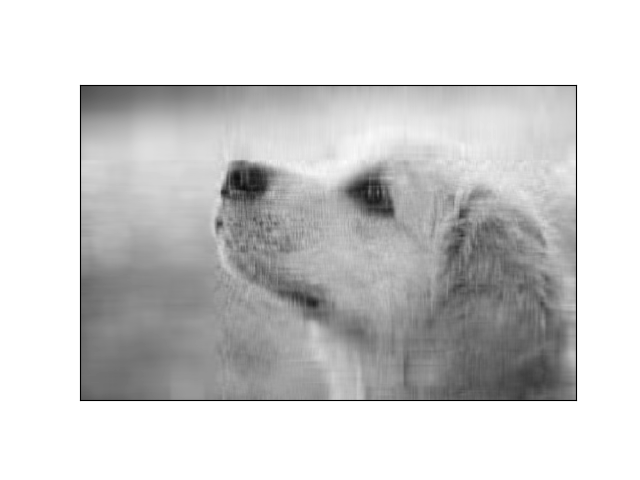
\includegraphics[scale=0.8]{problem1/Figure_1}
    	
    \subparagraph{$\bullet$}
    	The resulting equation for the fifth degree polynomial fit is 
    	\[
    	f(x) = 1.87 - 7.25x + 28.8x^2 - 58.7x^3 + 71.0x^4 - 25.2x^5.
    	\]
    	The 2-norm of the resulting error $E = ||b - Ax|| = 2.84\cdot10^{-5}$. Below is the resulting fitted curve.
    	
    	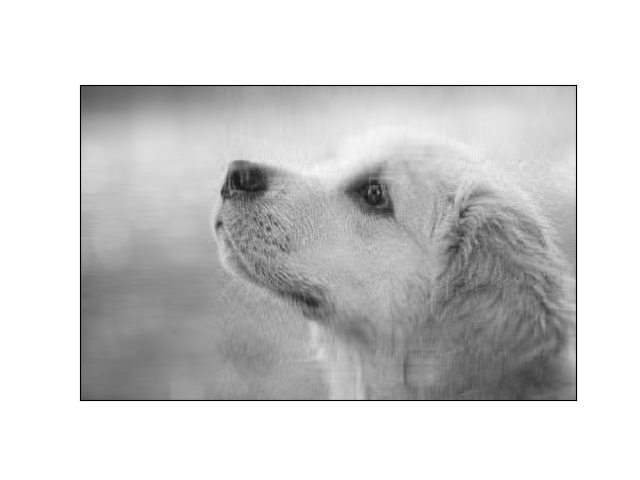
\includegraphics[scale=0.8]{problem1/Figure_2}
    	
    \subparagraph{$\bullet$}
    	single precision floats only store numbers from $10^{-38}$ up to $10^{38}$. When values carry essential information up to the sixth significant digit then being raised to anything over the fifth power will result in a lose of information. 
    	
    	From my code I found that fitting a curve up to the sixth degree polynomial resulted in significant error. 
    	
    
\paragraph{2.}
		
	

\end{document}












